\chapter{Descrição da proposta de projeto}

Conforme visto nos projetos correlatos, já foi desenvolvida uma gama de \textit{frameworks} RPC voltados para a comunicação entre processos e linguagens diferentes, cada qual com características únicas e diferentes objetivos. Foram propostas desde iniciativas para resolver as necessidades especificas de um conjunto de \emph{softwares} de um empresa, até conceitos mais genéricos que visam melhorar a comunicação de \textit{softwares} que usam o modelo cliente servidor. Entretanto, mesmo com essa variedade de propostas, identificamos a falta de uma solução simples direcionada para a comunicação remota na área de computação de alto desempenho \cite{soumagne2020advancing}. Em especial, em aplicações implantadas nos novos ambiente de nuvem, que incentivam desassociação de funcionalidades em microsserviços, que dependem mais da comunicação para compor sistemas mais distribuídos.

A partir dessas premissas, concebeu-se um \textit{framework} de RPC para atender às demandas de um ambiente de computação de alto desempenho, com foco no desempenho e na simplicidade de uso, e também com o intuito de reduzir a sobrecarga cognitiva de uso pelos desenvolvedores, uma vez que sistemas voltados para computação de alto desempenho já são suficientemente complexos \cite{lynn_addressing_2018}.

\section{Componentes}

O aRPC é composto por três grupos principais de componentes: o protocolo de transporte, o serializador e o gerador de código (compilador), o diagrama de blocos pode ser visto na Figura \ref{fig:arpc_components}.

\begin{figure}[ht]
    \centering
    \caption{Componentes do aRPC}
    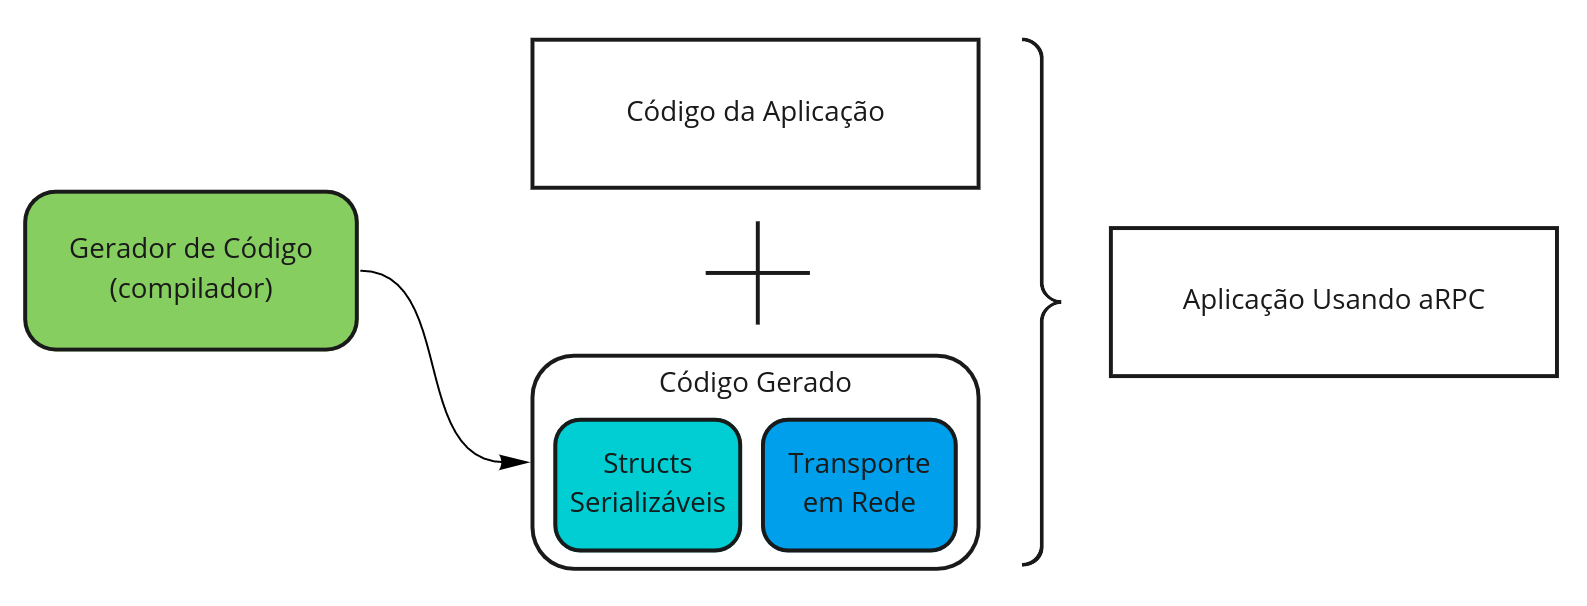
\includegraphics[width=\textwidth]{figuras/diagramas/cap3/componentes.png} 
    \label{fig:arpc_components}
\end{figure}

O protocolo de transporte é responsável pela comunicação entre os nós clientes e os servidores, efetuando o envio dos dados referentes aos argumentos dos clientes para os servidores e das respostas dos servidores de volta aos clientes.

O serializador é responsável por traduzir estruturas de dados complexas em sequências de bytes e transformar sequências de bytes de volta em estruturas de dados complexas \cite{newmarch_data_2017}. No contexto do RPC, o serializador também viabiliza a comunicação entre processos e linguagens distintas.

A geração de código é uma etapa opcional, realizada por um compilador. Alguns protocolos de RPC exigem a definição de uma especificação das estruturas de dados e dos procedimentos disponibilizados pelos serviços oferecidos \cite{ford_using_1995}. No caso do aRPC, o compilador é responsável por efetuar uma etapa de leitura do arquivo de especificação (também chamado de IDL - \textit{Interface Definition Language}) e em seguida gerar, na linguagem escolhida, o código que disponibiliza ao cliente as abstrações para efetuar chamadas de procedimentos, e para o servidor as interfaces necessárias para a implementação desses procedimentos. Desse modo, a serialização e transmissão de dados se torna transparente ao usuário.

\section{Protocolo de Transporte}

O aRPC tem como objetivo aprimorar a comunicação entre aplicações através da rede. Assim, se fez necessário a escolha de um protocolo de camada de transporte para melhor atender às características e necessidades de aplicações com foco em alto desempenho. Foram avaliados os prós e contras dos protocolos TCP, UDP e QUIC para utilização pelo \textit{framework} proposto.


\subsection{TCP}

Um dos protocolos originais da implementação da rede de computadores. Normalmente referido como TCP/IP \cite{cerf_protocol_1974}.
Desenvolvido em 1974 por Vint Cerf e Bob Kahn, o protocolo assegura a transmissão confiável de dados entre nós de uma rede de computadores. Para isso, implementa diversos mecanismos, como retransmissão de pacotes e controle de fluxo e congestão, que possibilitam um entrega de dados garantida, ordenada e com verificação de erros.

Enquanto essas características são de interesse para o funcionamento correto do aRPC, a complexidade de alguns desses métodos, da maneira que foram implementados no TCP, podem trazer desvantagens perceptíveis para alguns casos de uso almejados.

Um problema em especial está no funcionamento do mecanismo de garantia de entrega ordenada, implementada pelo TCP, para casos onde há conjuntos de dados independentes sendo transmitidos. Isso ocorre porque o TCP não tem como averiguar o conteúdo dos dados, o que obriga que todo pacote, mesmo que não relacionado com os demais, caso chegue ao destino fora de sua ordem, tenha que esperar por todos os pacotes anteriores \cite{scharf2006nxg03}. Essa situação leva ao aumento da latência na comunicação, especialmente nos casos onde problemas na camada de enlace possam ocasionar elevadas ocorrências de retransmissão de pacotes. Além disso, com o rápido crescimento da largura de banda da rede de comunicação, algumas deficiências no desempenho do TCP se tornaram aparentes. Mesmo com ajuste minuciosos dos parâmetros de conexões, o protocolo subutiliza substancialmente a largura de banda da rede disponível. 

Estes problemas de latência e eficiência do TCP podem ser contornados com o uso de multiplexação de conexão a nível de aplicação acompanhado de ajustes no algoritmo de controle de congestão \cite{rfc5681}.
Entretanto, algumas características intrínsecas de funcionamento do protocolo impedem um desempenho ótimo em diversos casos de interesse para um \textit{frameworks} RPC. O alto custo do mecanismo de \textit{handshake} em três etapas, especialmente entre nós já conhecidos, impossibilita o uso de multiplexação para conexões com vida útil curta, pois a latência introduzida resulta em desempenho médio pior do que com o uso de uma única conexão. Além disso, estratégias de \textit{slow start} do mecanismo de congestão impossibilitam o uso de novas conexões para a transmissão de uma pequena quantidade de dados, pois dificilmente ela sairia do período de \textit{slow start}, o que acarretaria em uso sub ótimo da largura de banda da conexão. A falta de multiplexação no nível de protocolo, impossibilita a reutilização dos sistemas de controle de congestão para múltiplas conexões entre os mesmos pares. Isso significa que a criação de novas conexões para cada transmissão de dado única sempre executa etapas que poderiam ser reaproveitadas. Logo, soluções de multiplexação de TCP que visem um bom desempenho, dependem do uso de estratégias de \emph{pool} de conexões, para alcançar um equilíbrio entre a latência decorrente do agrupamento de dados dissociados e a latência decorrente da manutenção de novas conexões TCP.

A criptografia dos dados em trânsito na rede é essencial atualmente, além de ser uma prática básica em diversos regulamentos de segurança em Tecnologia da Informação (TI). O TCP não apresenta nenhum recurso de segurança nativo. Isso pode ser contornado com o uso de protocolos sobre o TCP, como o TLS \cite{rfc5246}. Entretanto, a adição de TLS sobre TCP ocasiona um aumento na latência, devido à adição dos mecanismos de funcionamento necessários para esses protocolos extras.

Por fim, o TCP não foi escolhido como protocolo de transporte para o aRPC. Mesmo oferecendo diversas funcionalidades interessantes, as desvantagens demonstradas pelo protocolo vão contra vários pontos essenciais para o bom desempenho do \textit{framework}, em especial na questão de latência \cite{lakshman1997performance}. Trabalhar para contornar essas questões parece um acréscimo de complexidade e de escopo que escapam do propósito almejado, além de ir contra a premissa de manter a simplicidade de implementação.

\subsection{UDP}
\label{subsec:udp}

Um dos principais membros do conjunto de protocolos para a rede de computadores. Desenvolvido em 1980 por David P. Reed e padronizado na RFC768 \cite{postel_user_1980}, foi concebido com objetivo de ser um protocolo simples com um mínimo de mecanismos necessários para seu funcionamento sobre a camada IP. Tem como características principais um funcionamento independente de conexão, sem estado e sem garantias de entrega ou lógica para retransmissão, manutenção de ordem ou proteção contra duplicação. Sendo assim, o protocolo utiliza como unidade básica de transporte o datagrama, que são estruturas básicas de encapsulamento normalmente compostas por um cabeçalho e um bloco de dados. No cabeçalho é incluído a porta de origem e destino, além do seu tamanho e um código de verificação. Comparando-se com o pacote do TCP, que incluiu um cabeçalho consideravelmente maior e mais complexo, com informação referente a ordem, confirmação, informação para controle do fluxo de dado e controle de congestão.

Um protocolo simples traz diversas vantagens para certos aplicações e casos de uso. Em aplicações extremamente sensíveis à latência, a falta de um etapa de \textit{handshake} e de atrasos por retransmissão são grandes vantagens do UDP. Especialmente para dados que são resilientes à perda de certa quantidade de informação, nesse caso é possível citar transmissões de mídia em tempo real (VoIP, \textit{streaming} de video), na qual os \textit{codecs} de mídia já incluem mecanismos para correção de erro.

No caso específico para uso como protocolo de transporte de um \textit{framework} de chamada de procedimento remoto, a simplicidade do protocolo é muito interessante. A minimização da latência é importante já que, para ser um substituto para a execução de funções locais, requer um mínimo de atraso no estabelecimento de comunicação entre os pares. Entretanto, a falta de mecanismos básicos de garantia de entrega e ordenação de datagramas são problemáticos, particularmente a perda de dados relativos aos argumentos e respostas de procedimentos não é um comportamento que possa ser considerável válido no contexto do \textit{framework}.

É importante ressaltar que o UDP pode apresentar algumas restrições de vazão dependendo do ambiente de rede. Isso é feito como medida de proteção e prevenção contra alguns tipos de abusos e ataques específicos ao UDP. Dentre eles, os ataques de amplificação \cite{rossow2014amplification} se destacam como fonte de apreensão entre provedores de serviços, devido à facilidade com que podem ser explorados por agentes mal intencionados e à grande extensão do impacto que podem causar. Por isso, muitos provedores de serviços implementam limites nas taxas de transferência do UDP para impedir que suas infraestruturas seja usadas para promover esses tipos de ataques.

Sendo assim, o UDP não foi escolhido como protocolo de transporte para o aRPC. Já que seu funcionamento, por mais que seja simples e eficiente, não oferece funcionalidades básicas esperadas para que o \textit{framework} possa cumprir o funcionamento desejado. Além disso, a implementação dos mecanismos necessários para fornecer esses recursos sobre o protocolo, na camada de aplicação, foge da premissa inicial do aRPC de manter a simplicidade de implementação.

\subsection{QUIC}
\label{subsec:quic}

QUIC é um protocolo da camada de transporte, inicialmente desenvolvido por Jim Roskind no Google, implementado para aplicações da empresa a partir de 2012, como o \textit{Youtube} por exemplo \cite{langley_quic_2017}. Em 2015 foi submetido à IETF (\textit{Internet Engineering Task Force}) para ser padronizado de maneira aberta e independente.

Este protocolo se apresenta como um protocolo da camada de transporte, porém possui algumas características encontradas em protocolos da camada de aplicação, como a multiplexação de \textit{streams}, que pode ser encontrada no HTTP/2 \cite{de_saxce_is_2015}, além de utilizar o protocolo UDP, que também é um protocolo de camada de transporte.

Além da multiplexação de \textit{streams}, o QUIC ainda apresenta outras características interessantes para um RPC, tais como a conexão sendo realizada em 1-RTT, ao invés de 3-RTT presente no TCP; transmissão de dados em 0-RTT para conexões subsequentes para um servidor já conhecido; garantia de entrega de pacotes, possuindo ainda garantia de ordenação de dados apenas dentro uma mesma \textit{stream}. Dessa maneira evita o problema de \textit{Head-of-Line Blocking}, que ocorre quando um pacote de uma \textit{stream} é perdido e todas as \textit{streams} ficam esperando esse pacote ser reenviado, mesmo que as \emph{streams} sejam independentes, pelo modo como o TCP funciona, tais diferenças entre o QUIC e o TCP podem ser vistas em \cite{cook_quic_2017}. Cabe ainda ressaltar que o protocolo impõe que toda a comunicação de dados seja sempre efetuada utilizando TLS, desse modo, os dados trafegados são criptografados e é possível verificar a autenticidade de servidores e clientes remotos. Pela imposição do TLS, o protocolo já se organiza para que a troca de chaves criptográficas ocorra no \textit{handshake} inicial, sem a necessidade de efetuar mais de um RTT para preparar a comunicação criptografada, como é o caso do TCP.

Devido ao uso do UDP como base, os problemas de restrições presentes em alguns provedores de serviço podem afetar a performance do QUIC. Isso é um fato relevante, entretanto, o protocolo inclui um mecanismo para impedir falsificação de IPs de origem \cite{rossow2014amplification}, no qual clientes são atribuídos um \textit{token} autenticado pelo servidor que estão se comunicando para assegurar a propriedade do seu IP de origem. Isso impede que ataques de amplificação possam ocorrer, já que eles dependem da falsificação do IP de origem do datagrama. Sendo assim, por mais que atualmente alguns provedores possam ter regras que impactam o QUIC, espera-se que em breve essas restrições sejam removidas, dado a popularização do uso do protocolo.

O protocolo QUIC foi o escolhido como mecanismo de transporte do aRPC por conta das características apresentadas, essa escolha tem como objetivo diminuir o \textit{overhead} de transporte perante outros \textit{frameworks} que utilizam o TCP como base. Outras características que merecem destaque são a multiplexação de \textit{streams} que é usada pelo aRPC para separar chamadas de procedimentos distintas, possibilitando um código mais simples e abrindo mão da necessidade de armazenar IDs das requisições e respostas nos cabeçalhos. Além disso, do ponto de vista do balanceamento de carga onde um cliente pode se conectar a vários servidores distintos ao longo do tempo, as características de realizar a conexão em 1-RTT e envio de dados em 0-RTT para conexões subsequentes também se tornam características muito desejáveis para um \textit{framework} de RPC \cite{fatemian_why_2020}.

\section{Serializador}

Quando se trafega dados pela rede, é necessário que as duas pontas, cliente e servidor, estejam se comunicando no mesmo formato. Para o protocolo HTTP até a versão 1.1 por exemplo, esse formato é em texto simples, que é legível por humanos. A partir da versão 2 do HTTP e em outros protocolos, a comunicação é feita utilizando dados em formato binário. Um dos benefícios de se utilizar um formato pré-definido de comunicação entre as partes, é a possibilidade que cliente e servidor sejam implementados em linguagens e plataformas distintas \cite{slee_thrift_nodate}. 

Tanto cliente quanto servidor lidam diretamente com dados estruturados dentro de suas respectivas aplicações, para traduzir esses dados num formato binário a ser trafegado pela rede, se faz necessária uma etapa de serialização, ou seja, tradução das estruturas de dados para formato binário usado no transporte.

Para a implementação do trabalho, vários serializadores foram considerados, onde foram avaliados seus prós e contras, tais como o Protobuffers, Cap'n Proto e Colfer, descritos a seguir.

\subsection{Protobuffers}

Desenvolvido pelo Google como um formato para comunicação entre aplicações internas da empresa, tem o propósito de ser agnóstico à linguagem e à plataforma.

Ao utilizar Protobuffers, o usuário especifica as estruturas de dados que ele deseja serializar em um IDL com a extensão \textbf{.proto}, esse arquivo define as estruturas com capacidade de serialização. O usuário então passa esses arquivos para o compilador do Protobuffers, que irá gerar o código que define estruturas com capacidade de serialização na linguagem que o usuário escolher. Protobuffers suporta uma vasta gama de linguagens, como C, C++, Java, Python, Go, Ruby, Objective-C, C\#, JavaScript, Rust, entre outras.

Este serializador também oferece uma vasta gama de funcionalidades, como diversos tipos primitivos, mapas, enumerações, listas, tipos aninhados, campos opcionais, campos com valor padrão, entre outras. \cite{google_protobuffers_2008}. Um ponto negativo que se pode citar é a imposição do Protobuffers que cada campo nas \textit{structs} tenham um número identificador, tal número é incorporado na serialização, aumentando a quantidade de bytes na mensagem, que por consequência tende a aumentar o tempo de transmissão dos dados \cite{bagci_lightweight_2016}, entretanto, este fator é mitigado pelas estratégias de otimização na serialização.

Um ponto relevante a se destacar, é o alto acoplamento que este serializador tem com o \textit{framework} gRPC, também do Google, diversas funcionalidades do Protobuffers existem pra atender ao funcionamento do gRPC, assim como diversas \textit{funcionalidades} do gRPC se adéquam ao modo como o Protobuffers funciona. Tais motivos fizeram com que ele não fosse o serializador escolhido para o aRPC, dado que diversas funcionalidades que existem para atender as demandas do gRPC não se fazem necessárias para o propósito deste trabalho, introduzindo apenas um custo computacional desnecessário.

\includecode[Protobuffers]{Código exemplificando o uso da IDL do Protobuffers} {alg:grpc_doubletype.proto}{codigos/grpc/doubletype.proto}{}

No Código \ref{alg:grpc_doubletype.proto} pode ser conferido um exemplo de arquivo \textbf{.proto}. Nele são definidos os tipos de mensagem \textbf{NumberList} e \textbf{Result}, utilizados como argumentos de entrada e de saída, respectivamente, para o procedimento \textbf{Average} dentro do serviço \textbf{DoubleType}. Ressaltando-se também que pode haver partes adicionais específicas parada cada linguagem que os desenvolvedores estejam usando, um exemplo pode ser visto na linha com a variável \textbf{go\_package} que define o pacote a ser utilizado pelo arquivo de código base gerado para a linguagem Go. Tais detalhes exclusivos de cada linguagem podem ir gerando uma sobrecarga maior no arquivo de IDL ao longo do tempo, que potencialmente pode conter diversas linhas com elementos específicos de diversas linguagens, introduzindo uma complexidade desnecessária.

O Protobuffers ainda permite que os códigos gerados para serialização dos dados tenham otimizações específicas escolhidas pelo desenvolvedor na hora de executar o compilador para gerar os arquivos, tais como otimizações para comprimir os dados e trafegar uma menor quantidade de dados pela rede ou então para serializar os dados de maneira mais simplificada, de modo com que o custo computacional de processamento na serialização e desserialização seja menor. Entretanto, neste trabalho essas otimizações não foram avaliadas, o compilador do Protobuffers foi utilizado no modo padrão, onde o código gerado tende a ser eficiente de uma maneira mais genérica, sem nenhuma otimização voltada para casos específicos.

\subsection{Cap'n Proto}

Desenvolvido por Kenton Varda, um dos principais autores do Protobuffers após sua saída do Google, consolidado a partir de anos de experiência do criador ao trabalhar com sua criação anterior. O Cap'n Proto procura acertar em pontos cujo o autor julgou como problemáticos no Protobuffers. Um exemplo pode ser conferido no Código \ref{alg:example.cnp}

\includecode[CapnProto]{Código exemplificando o uso da IDL do Cap'n Proto} {alg:example.cnp}{codigos/example.cnp}{Adaptado da documentação da biblioteca em Go do Cap'n Proto (\url{https://github.com/capnproto/go-capnproto2/wiki/Getting-Started})}

Um dos conceitos chave do Cap'n Proto é o de zero cópias de memória nas etapas de serialização e desserialização dos dados. Os mesmos bytes operados na aplicação são os bytes que serão trafegados pela rede. Evitando assim o processamento dos dados na preparação da mensagem para envio.

O Cap'n Proto ainda apresenta diversas funcionalidades interessantes, tais como: a leitura incremental dos dados, que permite que uma mensagem possa começar a ser lida e desserializada antes ter sido recebida por completo; acesso aleatório, onde é possível ler um dos dados da mensagem sem a necessidade de desserializar os demais dados; o código gerado é pequeno, enquanto o Protobuffers gera código específico de serialização e desserialização para cada tipo de mensagem diferente, o Cap'n Proto utiliza chamadas otimizadas de sua própria biblioteca para lidar com essa parte, sendo que a própria biblioteca que é executada junto do programa também é pequena e otimizada.

Entretanto, apesar das funcionalidades interessantes, assim como o Protobuffers, o Cap'n Proto também é desenvolvido ao redor de um \textit{framework} de RPC próprio, com isso diversas funcionalidades existem apenas com o propósito de atender como o autor vislumbrou que o RPC deve funcionar, não atendendo tão bem às demandas deste trabalho. Além disso, para proporcionar um conjunto rico de funcionalidades e ao mesmo tempo proporcionar uma boa performance, o Cap'n Proto tomou certas escolhas de implementação que prejudicam a ergonomia na escrita de código, forçando os desenvolvedores a adequarem o resto da aplicação aos padrões do Cap'n Proto ou então ficar com o código heterogêneo no que se refere a manipulação de dados, que pode ser conferido no Código \ref{alg:example_cnp_bad_code}.

\includecode[Go]{Código exemplificando o meio de popular os objetos do Cap'n Proto} {alg:example_cnp_bad_code}{codigos/example_cnp_bad_code.go}{Adaptado da documentação da biblioteca em Go do Cap'n Proto (\url{https://github.com/capnproto/go-capnproto2/wiki/Getting-Started})}

\subsection{Colfer}

Desenvolvido por Pascal de Kloe, Colfer é um formato de serialização binária, otimizado em tamanho e velocidade.

O uso do Colfer se dá através de um compilador que processa aquivos \textbf{.colf}, escritos em uma IDL que discrimina as estruturas de dados a serem utilizadas,
e gera código fonte em uma das linguagens de programação suportadas. O código gerado é responsável por serializar as estruturas de dados previamente descritos em binário e vice-versa.

A linguagem IDL utilizada para descrição dos dados é derivada da sintaxe da linguagem Go, especificamente da sua definição de \textit{structs}, com a extensão de alguns tipos específicos definidos pelo Colfer, conforme pode ser visto no Código \ref{alg:exemple.colf}.

\includecode[Go]{Código exemplificando o uso da IDL do Colfer} {alg:exemple.colf}{codigos/exemple.colf}{Adaptado da documentação do Colfer (https://github.com/pascaldekloe/colfer)}

A vantagem do uso da sintaxe do Go é a fácil reutilização do ferramental já disponível para análise e manipulação de código textual, como o módulo AST, nativo do Go, que permite facilmente construir e interagir com a árvore sintática abstrata a partir do código fonte fornecido.

O Colfer define quatorze tipos de dados distintos. Entre eles, um tipo básico representando um booleano; quatro tipos básicos de inteiros não incluindo sinal, com resolução de 8, 16, 32 e 64 bits;
dois tipos de inteiros incluindo sinal, com resolução de 32 e 64 bits; dois tipos representativos de números com ponto flutuante, com resolução de 32 e 64 bits; 
um tipo que representa o registro de data/hora; um tipo que representa uma sequência variável de caracteres textuais; um tipo que representa uma sequência variável de dados binários; um tipo que representa um lista variável de qualquer um dos tipos disponíveis.

O formato de dados constitui-se por uma estrutura contendo zero ou mais definições de campos de valores, seguido por um byte de término 0x7f.
Somente são serializados campos de valores que representem dados não nulos, ou valores diferentes de zero.
Cada campo de valor é representado em memória no formato \textit{big-endian}, composto por um cabeçalho de 8 bits seguido por um campo de dado codificado em um formato de tamanho fixo ou de tamanho variável em base 128 (UBEB128) \cite{wang2017experimental}. 
Os 7 bits menos significativos do cabeçalho identificam o tipo do dado, de acordo com um índice internamente atribuído e o bit mais significativo é uma \textit{flag} reservada para uso específicos.

O formato do campo de dados de cada tipo é definido abaixo:

\begin{itemize}

    \item Booleanos somente são codificados quando verdadeiros, e não tem campo de dados, sendo definidos exclusivamente pelo cabeçalho.

    \item Inteiros de 8 bits sem sinal são codificados em formato fixo como 1 byte.

    \item Inteiros de 16 bits sem sinal, menores que 255, são codificados em formato fixo como 1 byte e com o valor do bit de \textit{flag} definido. Valores maiores são codificados em dois bytes.

    \item Inteiros de 32 bits sem sinal, menores que 0x200000 são codificados como inteiros de comprimento variável. Valores maiores são codificados em formato fixo como 4 bytes e com o valor do bit de \textit{flag} definido.

    \item Inteiros de 64 bits sem sinal, menores que 0x2000000000000 são codificados como inteiros de comprimento variável. Valores maiores são codificados em formato fixo como 8 bytes e com o valor do bit de \textit{flag} definido.

    \item Inteiros de 32 e 64 bits com sinal são codificados como inteiros de comprimento variável, onde o valor do bit da \textit{flag} representa o sinal. No caso de inteiros de 64 bits maiores que 0x8000000000000000, o ultimo byte da codificação UBEB128 não é codificado pois ele sempre será 0x1.

    \item Números de ponto flutuante são codificados conforme a IEEE754 \cite{noauthor_ieee_2019}.

    \item Registros de data/hora podem ser codificados de dois modos:
\begin{itemize}
	\item Inteiro de 32 bits sem sinal representando o número de segundos decorridos a partir de 00:00:00 UTC, quinta-feira, 1 de janeiro de 1970
    \item Inteiro de 64 bits sem sinal representando o número de segundos decorridos a partir de 00:00:00 UTC, quinta-feira, 1 de janeiro de 1970, e com o valor do bit de \textit{flag} definido
\end{itemize}

Ambos os formatos são seguidos de um inteiro de 32 bits (onde somente os primeiros 30 bits são utilizados) sem sinal representando a fração de nanosegundos.

    \item Listas são codificadas por um inteiro de tamanho variável representando o número de entradas(\textbf{N}), seguido por \textbf{N} campos de valores representando os dados da lista.

    \item Sequências de bytes são definidas por por um inteiro de tamanho variável representando o número de entradas(\textbf{N}), seguido por \textbf{N} bytes descrevendo o dado original.

    \item Textos seguem a mesma codificação de sequências de bytes, com os caracteres codificados em UTF-8 \cite{noauthor_unicode_2010}.

\end{itemize}

O código gerado pelo Colfer, a partir do arquivo de definições, é livre de dependências e somente utiliza as funcionalidades nativas de cada linguagem suportada para codificar e decodificar as estruturas de dados.
Orientado para simplicidade e com um mínimo de \textit{overhead} para realizar as tarefas necessárias para serialização, o código gerado não considera como o dado será transportado, sendo de responsabilidade do desenvolvedor interagir com os métodos disponibilizados. 

O Colfer se destaca entre os serializadores analisados por diversas vantagens: simplicidade e extensibilidade que permitem fácil integração de suas funcionalidades; não necessita de dependências externas, com todas as funcionalidades sendo oferecidas pelo compilador; geração de código nativo na linguagem alvo, com foco no alto desempenho, sem sacrifício de segurança. Esse conjunto de características fez com que o Colfer fosse o serializador escolhido para uso no aRPC.

\section{Arquitetura do aRPC}

A arquitetura do aRPC é inspirada pela arquitetura do gRPC e do HPRPC \cite{bagci_lightweight_2016}, entretanto, foram feitas algumas alterações. 

\begin{figure}[ht]
    \centering
    \caption{Arquitetura do aRPC}
    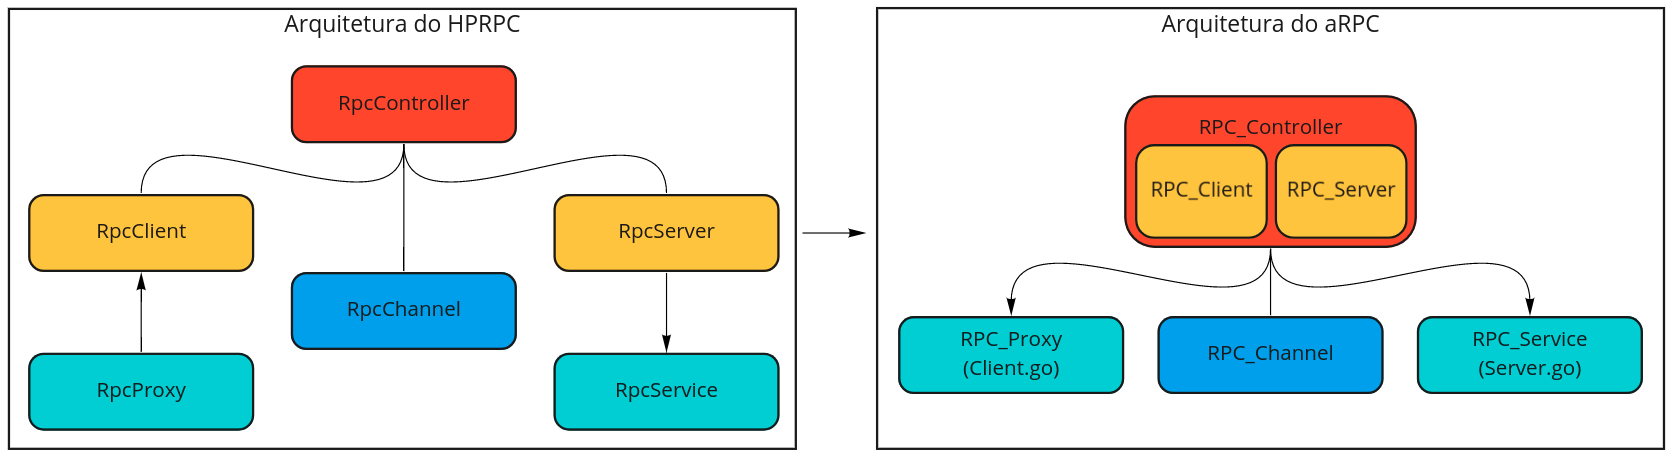
\includegraphics[width=\textwidth]{figuras/diagramas/cap3/arquitetura.png} 
    \label{fig:arpc_arquitetura}
\end{figure}

Primeiramente, o \textbf{RPC\_Client} e \textbf{RPC\_Server} que definem as funções de envio e recebimento foram incorporadas no \textbf{RPC\_Controler}. O \textbf{RPC\_Proxy} se refere ao código gerado para clientes e \textbf{RPC\_Service} para servidores, dessa forma são análogos aos arquivos \textbf{Client.go} e \textbf{Server.go} gerados pelo compilador do aRPC para cada serviço. Além disso, o \textbf{RPC\_Channel} foi implementado usando interfaces baseadas na implementação do QUIC no Go, facilitando dessa forma a construção do controlador a partir das facilidades do QUIC, como a multiplexação de \textit{streams}. A implementação do \textbf{RPC\_Channel} no aRPC parte de interfaces que possibilitam o uso de outro protocolo como base, como HTTP/2 ou TCP. Essas implementações foram deixadas como recomendação de trabalhos futuros, para uma melhor comparação dos protocolos de transporte isoladamente.

O seguintes critérios foram considerados fundamentais na definição do protocolo: ele deveria ser rápido na serialização, na desserialização e no transporte; capaz de produzir binários pequenos para envio; não comprometer demais a ergonomia de desenvolvimento normal da linguagem e; finalmente, ser simples. Atualmente a única linguagem suportada é Go, entretanto, como o protocolo é simples, sua portabilidade e funcionamento em conjunto com outras linguagens é de fácil implementação.

Quanto ao envio de mensagens, optou-se por usar 1 byte inicial que define o tamanho do cabeçalho, em seguida dentro do cabeçalho existe um campo que define o tamanho dos dados enviados, com essas duas informações ambas as pontas (cliente e servidor) são capazes de montar a requisição e de serializar e desserializar cabeçalho e dados. Essa arquitetura de mensagem foi definida pensando facilitar a desserialização e também em usar a característica do Colfer de serializar somente os dados necessários, reduzindo a sobrecarga de envio do cabeçalho e dos dados em cada mensagem.

É interessante notar que, do modo como o controlador foi implementado, é possível rodar o cliente e o servidor de serviços aRPC simultaneamente. Com uma única instância de \textbf{aRPC\_Controller} é possível consumir múltiplos serviços e ao mesmo tempo oferecer serviços a múltiplos clientes. 

Anteriormente, foi dito que o aRPC possui um gerador de código, este compilador é responsável por gerar \textit{boilerplates} que são utilizados para integrar os serializadores com o controlador e fazer serialização e transportes serem transparentes do ponto de vista do usuário. Um exemplo de código gerado para o cliente pode ser conferido no Código \ref{alg:arpc_compiler_client.go}, enquanto o lado do servidor pode ser visto no Código \ref{alg:arpc_compiler_server.go}

\includecode[Go]{Código gerado pelo compilador do aRPC para o \textit{client} de um serviço simples} {alg:arpc_compiler_client.go}{codigos/compilador/client.go}{}

\includecode[Go]{Código gerado pelo compilador do aRPC para o \textit{server} de um serviço simples} {alg:arpc_compiler_server.go}{codigos/compilador/server.go}{}

\subsection{Channel}

O módulo \textbf{aRPC\_Channel} é responsável por abstrair para o controlador qual protocolo de transporte será usado na comunicação aRPC. Neste trabalho foi implementado o \textbf{QUIC\_Channel}, fornecendo uso do aRPC através de QUIC. No entanto, a implementação de \textit{channels} para outros protocolos de transporte é de fácil construção, necessitando apenas da implementação das interfaces a seguir: 

\begin{figure}[ht]
    \centering
    \caption{Relação das interfaces de um channel no aRPC}
    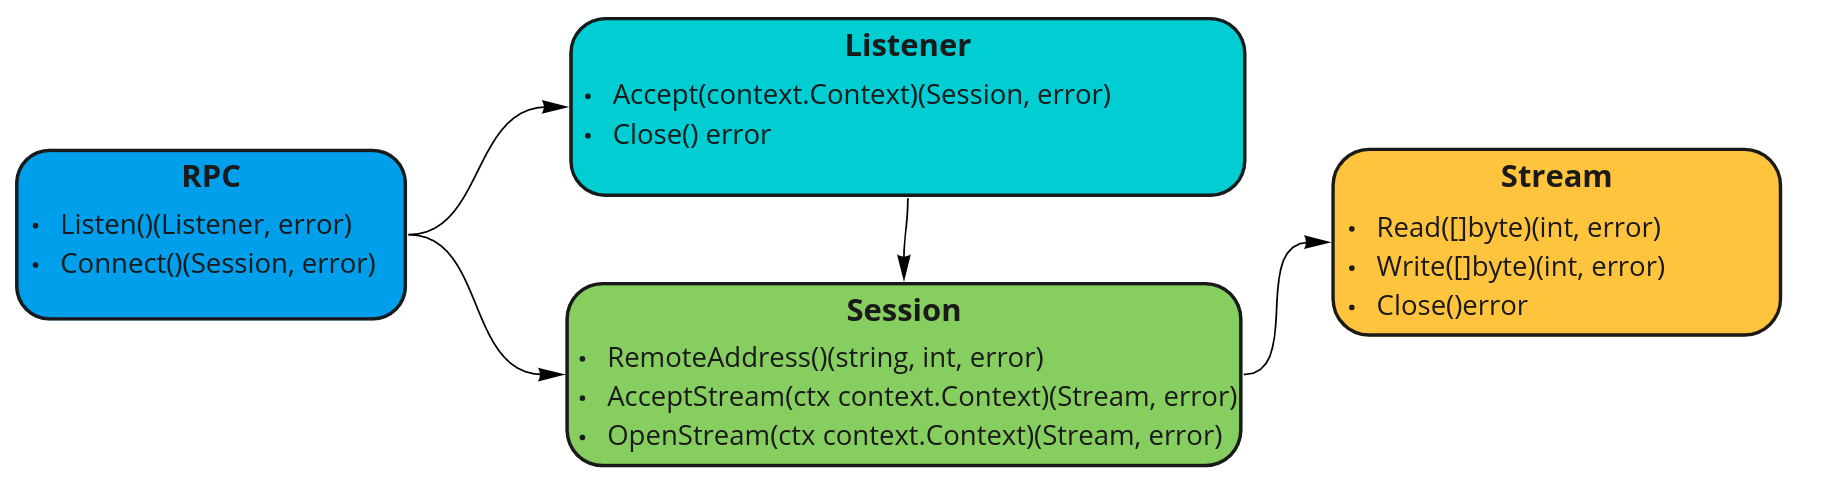
\includegraphics[width=\textwidth]{figuras/diagramas/cap3/interfaces.png} 
    \label{fig:arpc_channel_interfaces}
\end{figure}

\subsubsection{Interface channel.RPC}

O \textbf{channel.RPC} é a interface de definição raiz do \textit{channel} e deve fornecer duas funções, \textbf{Listen} e \textbf{Connect}. As funções e suas respectivas definições estão listadas abaixo:

\begin{itemize}
	\item \textbf{Listen( )(Listener, error)} - Função responsável por iniciar o recebimento de conexões, retornando em caso de sucesso um \textbf{Listener}, que é uma outra interface que deve ser implementada e cuja definição será vista na subseção seguinte.
	\item \textbf{Connect( )(Session, error)} - Função que executa para um cliente a conexão com um servidor que tenha executado o método \textbf{Listen} previamente. Retornando assim uma \textbf{Session} que é uma interface deve ser implementada e cuja definição será vista a seguir.
\end{itemize}

\subsubsection{Interface channel.Listener}

A interface \textbf{channel.Listener} provê ao \textbf{aRPC\_Controller} as funções referentes ao servidor e um meio de receber novas conexões de clientes. Dessa forma, essa interface define os métodos abaixo:

\begin{itemize}
	\item \textbf{Accept(context.Context)(Session, error)} - Função que espera novas conexões e em seguida retorna uma sessão para conexão com o cliente. como dito anteriormente, \textbf{Session} é uma das interfaces que devem ser implementadas e cuja definição será vista mais à frente.
	\item \textbf{Close( ) error} - Essa função fecha o \textit{listener} para recebimento de novas conexões, e consequentemente, o servidor associado a ele.
\end{itemize}

\subsubsection{Interface channel.Session}

A interface \textbf{channel.Session} é responsável por fornecer ao \textbf{aRPC\_Controller} acesso às propriedades da conexão e também faz a abertura ou recebimento de \textit{streams} de dados. No aRPC cada chamada de procedimento remoto abre uma nova \textit{stream} que  é fechada ao fim da execução do procedimento. Uma observação importante é que fechar a \textit{stream} não implica em fechar a conexão, já que a \textit{stream} é um mecanismo lógico. A interface \textbf{channel.Session} define assim, os métodos abaixo:

\begin{itemize}
	\item \textbf{RemoteAddress( )(string, int, error)} - Essa função retorna para o nó em questão (cliente ou servidor) o endereço e porta usados para conexão com o nó remoto.
	\item \textbf{AcceptStream(ctx context.Context)(Stream, error)} - Função bloqueante, responsável por liberar o fluxo quando um nó remoto abre uma nova \textbf{Stream} e retorna-lá. \textbf{Stream} também é uma interface que deve ser implementada e e cuja definição será vista adiante.
	\item \textbf{OpenStream(ctx context.Context)(Stream, error)} - Inicia uma nova \textbf{Stream} dentro da \textbf{Session} atual. Como dito anteriormente, \textbf{Stream} é uma interface que deve ser implementada e cuja definição será vista adiante.
\end{itemize}

\subsubsection{Interface channel.Stream}

A interface \textbf{channel.Stream} é a última das interfaces que deve ser implementada para disponibilizar um novo \textbf{Channel}, nela estão definidas funções de envio e leitura de bytes e também um método para fechar a \textbf{Stream}. A interface \textbf{channel.Stream} define os seguintes métodos:

\begin{itemize}
	\item \textbf{Read([ ]byte)(int, error)} - Lê a partir da \textbf{Stream} dados enviados pelo nó remoto.
	\item \textbf{Write([ ]byte)(int, error)} - Escreve os dados contidos em um \textbf{[]byte} na \textbf{Stream} para leitura pelo nó remoto.
	\item \textbf{Close( )error} - Essa função fecha a \textbf{Stream} em questão e no caso do aRPC finaliza uma execução de um procedimento de RPC.
\end{itemize}

\subsubsection{Implementação do \textbf{QUIC\_Channel}}

No estado atual, o \textit{framework} disponibiliza um \textbf{Channel} que usa QUIC como protocolo de transporte nativo, e essa implementação pode ser vista tanto no github do aRPC (\url{https://github.com/almeida-raphael/arpc}) quanto no Código \ref{alg:arpc_quic_channel_rpc.go}, Código \ref{alg:arpc_quic_channel_listener.go}, Código \ref{alg:arpc_quic_session.go} e Código \ref{alg:arpc_quic_stream.go}. A implementação atual disponibiliza \textit{streams} multiplexadas, \textit{handshake} de baixo custo computacional, entre outros benefícios associados ao uso do QUIC como protocolo de transporte. Como as interfaces foram desenhadas baseadas em conceitos do QUIC, isso facilitou muito sua implementação como \textbf{Channel} inicial disponibilizado no \textit{framework}. Dessa forma, pode-se observar que o código é bastante semântico e curto. O QUIC foi escolhido como \textbf{Channel} nativo por apresentar características que indicavam ser uma ótima escolha inicial para o protocolo, que por definição fornece criptografia e verificação de autenticidade de origem com TLS, além de ser um protocolo de simples utilização.

\includecode[Go]{Implementação da interface channel.RPC para QUIC} {alg:arpc_quic_channel_rpc.go}{codigos/arpc/channels/quic_rpc.go}{}

\includecode[Go]{Implementação da interface channel.Listener para QUIC} {alg:arpc_quic_channel_listener.go}{codigos/arpc/channels/quic_listener.go}{}

\includecode[Go]{Implementação da interface channel.Session para QUIC} {alg:arpc_quic_session.go}{codigos/arpc/channels/quic_session.go}{}

\includecode[Go]{Implementação da interface channel.Stream para QUIC} {alg:arpc_quic_stream.go}{codigos/arpc/channels/quic_stream.go}{}


\subsection{Controler}

O \textbf{aRPC\_Controller} é o bloco central que disponibiliza métodos de envio e recebimento de requisições de RPC. Ele é responsável por controlar tamanhos de mensagens, gerar e ler cabeçalhos, serializar e desserializar dados, registrar serviços e procedimentos oferecidos e dar ao \textit{framework} formas de enviar e receber respostas RPC, sem se preocupar com a etapa de transporte. 

No aRPC, a camada do \textbf{Controler} não é diretamente usada pelo usuário para registrar e chamar serviços e procedimentos, essa camada é invocada pelo código gerado pelo compilador, o que torna a execução do aRPC e o fornecimento de serviços e procedimentos transparentes ao usuário. Dessa forma, o transporte e eventual execução remota não impactam significativamente a estrutura normal da linguagem. É um dos fundamentos do aRPC manter o usuário dentro das características da linguagem que a aplicação está sendo desenvolvida e oferecer mais ergonomia que algumas das soluções disponíveis no mercado.

O \textbf{Controller} fornece em sua API pública o seguinte conjunto de funções:

\begin{itemize}
	\item \textbf{StartServer} - Função responsável por iniciar o servidor e disponibilizá-lo para recebimento de requisições RPC.
	\item \textbf{StartClient} - Função que inicia a conexão do cliente com os respectivos servidores e o prepara para invocar de forma remota os procedimentos e serviços oferecidos pelos servidores alvo.
	\item \textbf{RegisterService} - Função usada pelo gerador de código para registrar serviços e procedimentos implementados por um servidor aRPC.
	\item \textbf{SendRPCCall} - Função que é chamada pelo gerador de código para efetuar envio de requisições RPC a partir do cliente, esta função cuida da serialização, envio, recebimento de resposta e desserialização dos dados.
	\item \textbf{SendData} - Função usada pelo gerador de código para efetuar o envio de resposta de um RPC executado já com dados serializados para o cliente, essa função se relaciona intimamente com o registro e invocação de serviços e procedimentos.
\end{itemize}

\subsection{Código Gerado}

O gerador de código é responsável por tornar transparente ao usuário o transporte e execução remota do RPC. O aRPC tem um foco grande em ergonomia, sendo assim, não é exigido que usuário construa o \textit{boilerplate} para serialização, envio de dados e interação com o \textbf{Controller}. Todo esse código é gerado por uma ferramenta de CLI e seu funcionamento  é descrito em detalhes à frente.

O gerador de código produz uma nova função para cada serviço a ser invocado pelo cliente, empacotando a função \textbf{controller.SendRPCCall} em chamadas específicas definidas no arquivo de IDL, cuidando da sua declaração e tipagem, tornando dessa forma a definição do RPC transparente ao cliente. Um exemplo de IDL do aRPC pode ser conferido no Código \ref{alg:arpc_compiler_idl.go}.

\includecode[Go]{Exemplo de IDL usada compilador do aRPC para definição de um serviço simples} {alg:arpc_compiler_idl.go}{codigos/compilador/idl.arpc.go}{}

Existem  no servidor dois blocos de código a serem compostos pelo gerador: o primeiro consiste nas funções oferecidas pelo serviço declarado na IDL e sua interface; o segundo refere-se à função de registro de serviço disponibilizada ao cliente. Para construir o primeiro grupo, são gerados códigos que desserializam os argumentos de execução e chamam a função implementada pelo nó. Em seguida, os dados são serializados e enviados usando a função \textbf{controller.SendData} para cada uma das funções definidas na IDL. Por fim, para o último grupo, é gerada uma função de registro que recebe uma \textit{struct} que implementa a interface disponibilizada para o servidor do serviço. Por último, essa função registra todos os procedimentos e o serviço no \textbf{Controler}. Os serviços são registrados com a função hash \textbf{FNV-1a} para facilitar o transporte de seu id como \textbf{int32} e os procedimentos de um serviço registrados com \textbf{uint16} sequencial de seus procedimentos na ordem de geração. 

Exemplos de código gerados para clientes e servidores podem ser conferidos no Código \ref{alg:arpc_compiler_client.go} e Código \ref{alg:arpc_compiler_server.go} definidos anteriormente.

\subsection{Mensagens}

As mensagens de requisição de aRPC e de resposta são construídas da seguinte forma: o primeiro byte é responsável pelo tamanho do cabeçalho a ser lido. Em seguida, um cabeçalho de tamanho variável é enviado. Por fim, o corpo da mensagem, que tanto podem ser os argumentos para requisição do aRPC, quanto pode ser a resposta, dependendo do cabeçalho. 

\begin{figure}[ht]
    \centering
    \caption{Diagramação das mensagens do aRPC}
    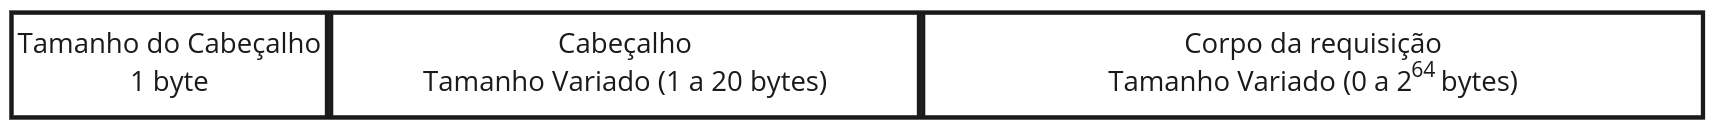
\includegraphics[width=\textwidth]{figuras/diagramas/cap3/arpc_message.png} 
    \label{fig:arpc_messages}
\end{figure}

Além disso, os dados do corpo são serializados para bytes através do sistema de serialização do aRPC. O cabeçalho carrega informações referentes ao serviço, procedimento e tipo de mensagem, como pode ser visto a seguir.

\subsubsection{Cabeçalho}

O cabeçalho do aRPC é composto por quatro campos, \textbf{MessageType} que é um \textbf{uint8}, \textbf{ServiceID} que é do tipo \textbf{uint32}, \textbf{ProcedureID} que é \textbf{uint16} e por fim o \textbf{PayloadSize} que é um \textbf{uint64}.

\begin{figure}[ht]
    \centering
    \caption{Diagramação do cabeçalho do aRPC}
    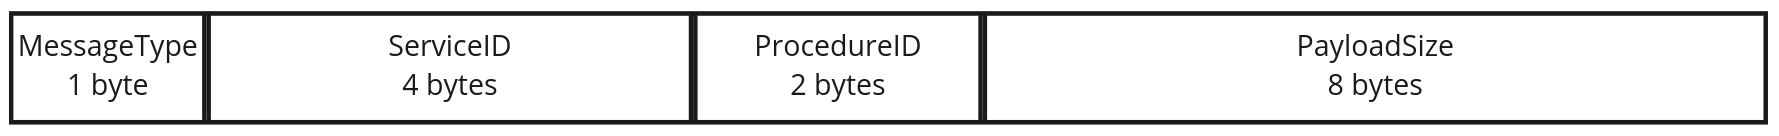
\includegraphics[width=\textwidth]{figuras/diagramas/cap3/arpc_header.png} 
    \label{fig:arpc_header}
\end{figure}

\begin{figure}[ht]
    \centering
    \caption{Diagramação do cabeçalho serializado pelo Colfer}
    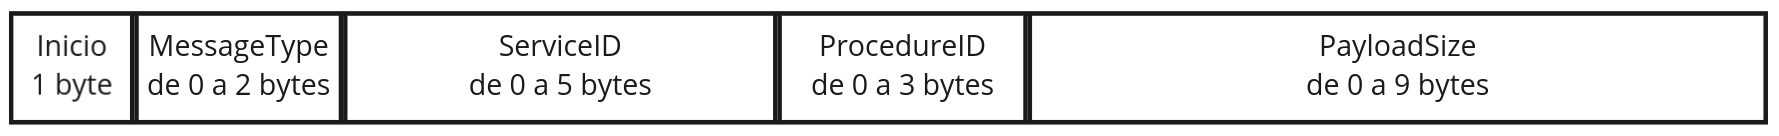
\includegraphics[width=\textwidth]{figuras/diagramas/cap3/arpc_header_colfer.png} 
    \label{fig:arpc_header_colfer}
\end{figure}

É possível observar, através da comparação da Figura \ref{fig:arpc_header} com a Figura \ref{fig:arpc_header_colfer}, que no processo de serialização pelo Colfer, devido às estruturas necessárias a serialização, pode-se diminuir ou aumentar o tamanho do cabeçalho em relação à definição dos tipos de campos. Por isso, apesar da soma dos tamanhos dos campos no cabeçalho ser 15 bytes, o tamanho serializado varia de 1 a 20 bytes, dependendo dos valores enviados.

O campo \textbf{MessageType} define o tipo de requisição, que pode ser \textbf{Call}, \textbf{Result} ou \textbf{Error}, com seus IDs sendo 0, 1 e 2, respectivamente. \textbf{Call} é o tipo utilizado em uma requisição aRPC, nesse caso o conteúdo do corpo são os argumentos. \textbf{Result} é o tipo utilizado na resposta de uma requisição aRPC e nesse caso o conteúdo do corpo é a resposta. Por fim se o tipo for \textbf{Error}, o conteúdo do corpo é o erro lançado pelo procedimento executado no servidor.

O \textbf{ServiceID} descreve qual é o serviço de destino da requisição e, em conjunto com o \textbf{ProcedureID}, informa ao \textbf{Controller} qual é o procedimento que deve ser executado.

O \textbf{PayloadSize} informa ao \textbf{Controller} qual é o tamanho do dado serializado a ser recebido, sendo usado para controlar se a mensagem já foi recebida completamente, ou se ainda existem bytes faltando.

Uma característica interessante do cabeçalho é que ele tem tamanho variável apesar de seus campos e tipos serem fixos. O Colfer garante que somente dados preenchidos e diferentes dos valores padrão serão serializados, além disso, estruturas distintas de dados são utilizadas ao se serializar, para diminuir o tamanho no binário final, dependendo do tipo e tamanho do dado. Tais fatores forçam o \textbf{Controller} a receber o tamanho do Cabeçalho como primeiro dado para saber o momento de desserializá-lo.

As mensagens no aRPC são enviadas em pares em \textbf{Streams} individuais, ou seja, para cada procedimento invocado, uma nova \textbf{Stream} é criada e tanto requisição quanto resposta trafegam na mesma \textbf{Stream}. O uso da \textbf{Stream} como mecanismo de associação de requisição com resposta dispensa a necessidade do uso de campos de ID no cabeçalho e facilita a implementação do protocolo, gerando um cabeçalho mais enxuto quando comparado ao HPRPC \cite{bagci_lightweight_2016}.

\section{Gerador de código}

O aRPC implementa um gerador de código que processa uma \textit{Interface Definition Language} (IDL), com gramática igual à linguagem Go, para gerar as implementações dos serviços.

O gerador é dividido em cinco etapas, como pode ser visto na Figura \ref{fig:arpc_compiler_pipeline}. 

\begin{figure}[ht]
    \centering
    \caption{Fluxo de compilação do CLI do aRPC}
    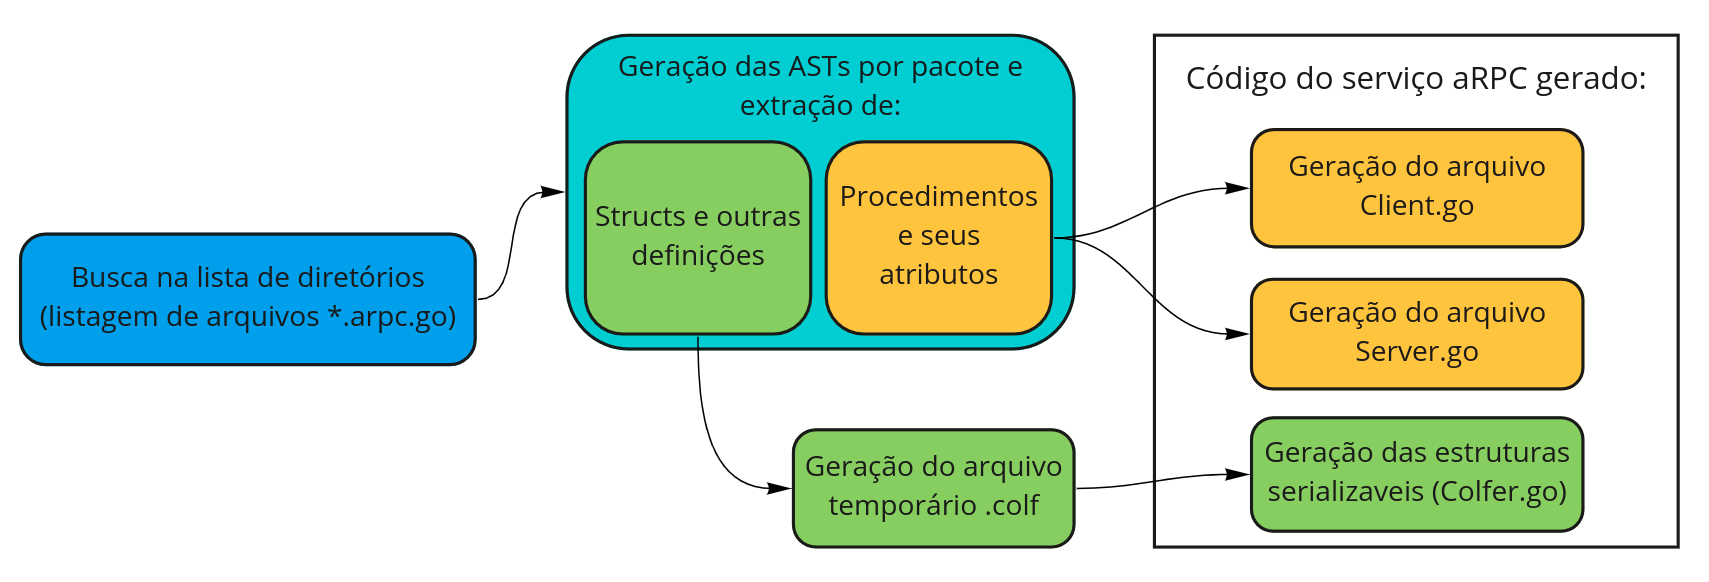
\includegraphics[width=\textwidth]{figuras/diagramas/cap3/arpc_compilador.png} 
    \label{fig:arpc_compiler_pipeline}
\end{figure}

Na primeira etapa, o compilador percorre uma lista de diretórios, a partir de um caminho fornecido pelo usuário, buscando pacotes de serviços e lendo suas respectivas definições nos arquivos de tipo \textit{*.arcp.go}. Em seguida, uma árvore sintática, onde são identificados os procedimentos remotos e seus atributos, é gerada a partir das definições de interfaces. Depois, as definições dos tipos de dado são extraídas, sendo gerado um arquivo \textit{.colf}, sobre o qual é invocado o gerador de código do Colfer, de modo a derivar as \textit{structs} e suas correspondentes funções de serialização. Na quarta etapa, é gerado o arquivo \textbf{Client.go} que integra o processo de serialização dos argumentos e respostas com o controlador do aRPC para uso pela aplicação cliente. Por fim, é construído o arquivo \textbf{Server.go} para uso na aplicação servidor, que disponibiliza uma função para registrar as implementações dos procedimentos do serviço no controlador, além de integrar a serialização de seus argumentos e respostas.

Existem algumas exigências no protocolo do aRPC que devem ser seguidas pelos arquivos de definição de interface dos serviços. Primeiro, todo procedimento deve retornar um parâmetro de erro, mesmo que a implementação da função não gere erros. Isso ocorre porque o transporte em rede e a execução remota podem ocasionar erros durante a sua execução, os quais devem ser tratados e informados ao cliente. Além disso, os argumentos e resposta devem implementar a interface \textit{Serializable} do aRPC, o que impede o uso de tipos básicos, que precisam ser encapsulados por \textit{structs}. Por fim, somente é permitido um argumento e uma resposta por procedimento. 

Essas restrições existem para facilitar a implementação do gerador de código e controlador e, por mais que acarretem em menor flexibilidade e funcionalidades quando comparado com outros protocolos RPC de uso geral, é possível que em um trabalho futuro elas possam ser removidas a fim de melhorar a ergonomia do aRPC. Contudo, não existe nenhum empecilho severo sobre o usuário e programador devido as essas limitações, e a maioria delas podem ser contornadas devido à flexibilidade do uso das \textit{structs} de entrada e saída que permitem maior liberdade na quantidade e tipos de argumentos e resposta.

O gerador de código foi disponibilizado como uma aplicação de \textit{command line interface} (CLI). Dessa forma, é possível instalá-lo no sistema usando somente uma linha no terminal e seu uso é fácil para novos desenvolvedores. A documentação de uso e instalação está disponível no repositório do código fonte da ferramenta no Github (\url{https://github.com/almeida-raphael/arpc\_code\_generator}).

\subsection{Varredura dos Diretórios e Pacotes}

Na etapa de varredura dos diretórios e pacotes, o gerador de código do aRPC recebe o caminho fornecido pelo usuário e efetua uma varredura recursiva dos diretórios procurando por arquivos de IDL \textbf{*.arpc.go}. Após obtenção da lista de arquivos, é feito um agrupamento do conteúdo dos arquivos de IDL em seus respectivos pacotes. Então, itera-se em cada pacote e, utilizando sua IDL, é construida uma \textit{Abstract Syntax Tree} (AST).

\subsection{Leitura da árvore Sintática e Geração de \textit{Structs}}

A AST é utilizada para identificar os procedimentos a serem disponibilizados pelo serviço, além de seus nomes, nomes e tipos de argumentos e tipo de retorno. Para isso, percorrem-se os nós da AST e para cada nó é verificado o seu tipo, para encontrar uma sequência de símbolos que caracterizem um procedimento \cite{zaytsev_parsing_2014}. Para cada procedimento são determinados seus atributos, especialmente seu nome, o nome dos argumentos, o tipo dos argumentos e o tipo de retorno. Depois de devidamente identificados e processados, os nós referentes aos procedimentos são removidos da AST e os remanescentes são traduzidos novamente em um arquivo temporário \textbf{.colf}.

\begin{figure}[ht]
    \centering
    \caption{Exclusão do nó de função da AST do Go}
    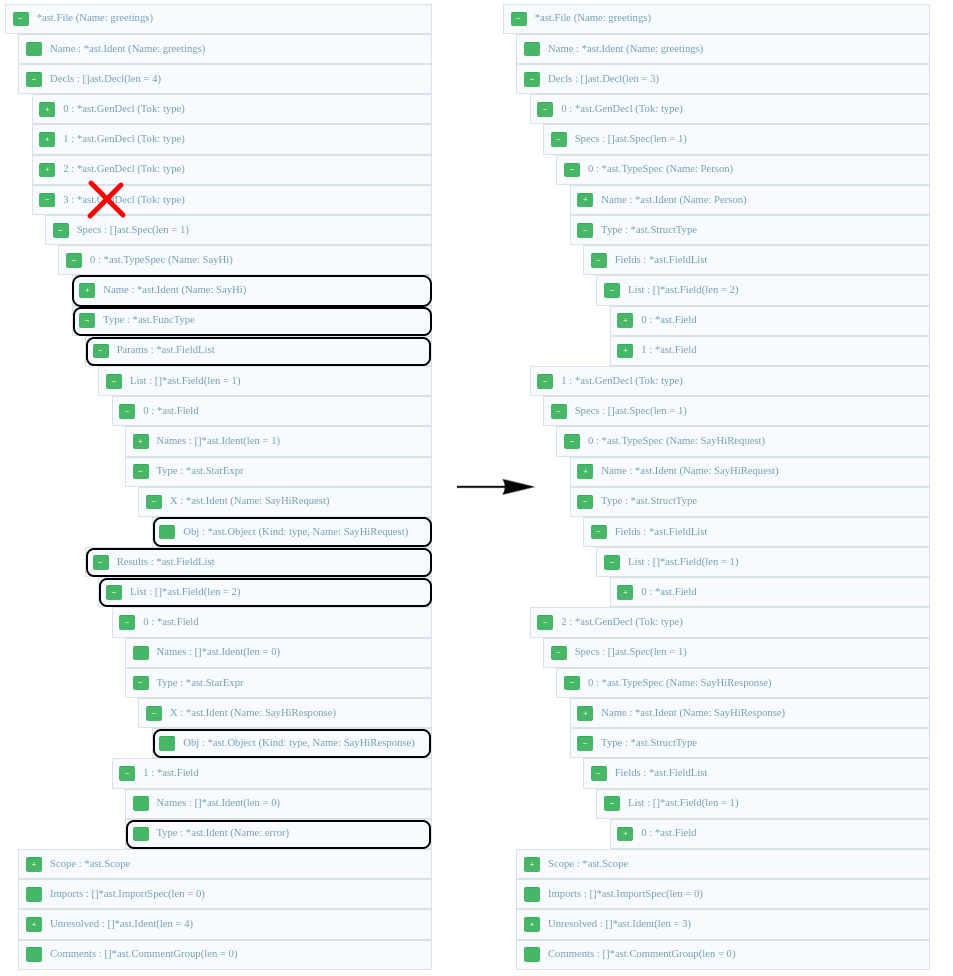
\includegraphics[width=\textwidth]{figuras/diagramas/cap3/ast.png}
    \label{fig:arpc_ast_function_removal}
\end{figure}

Os arquivos \textbf{.colf} são arquivos de IDL usados pelo Colfer, o serializador do aRPC, para gerar as \textit{structs} relevantes aos serviços e procedimentos definidos nos arquivos \textbf{*.arpc.go}. Uma vez construídos os arquivos temporários \textbf{*.colf}, o gerador de código do aRPC invoca a ferramenta de \textit{command line interface} (CLI) do Colfer, passando como argumento o local onde devem ser gerados os pacotes, tamanhos máximos de estruturas e listas, e o arquivo \textbf{*.colf} de entrada. Esse procedimento é repetido para cada pacote identificado e processado nos arquivos \textbf{*.arpc.go}.

\subsection{Geração de código aRPC para clientes}

A geração do código dos procedimentos do serviço para o arquivo \textbf{Client.go} precisa somente dos dados referentes aos procedimentos disponíveis, o nome do pacote de origem e \textit{templates} para geração de código.

\begin{figure}[ht]
    \centering
    \caption{Processo de geração do arquivo Client.go aRPC}
    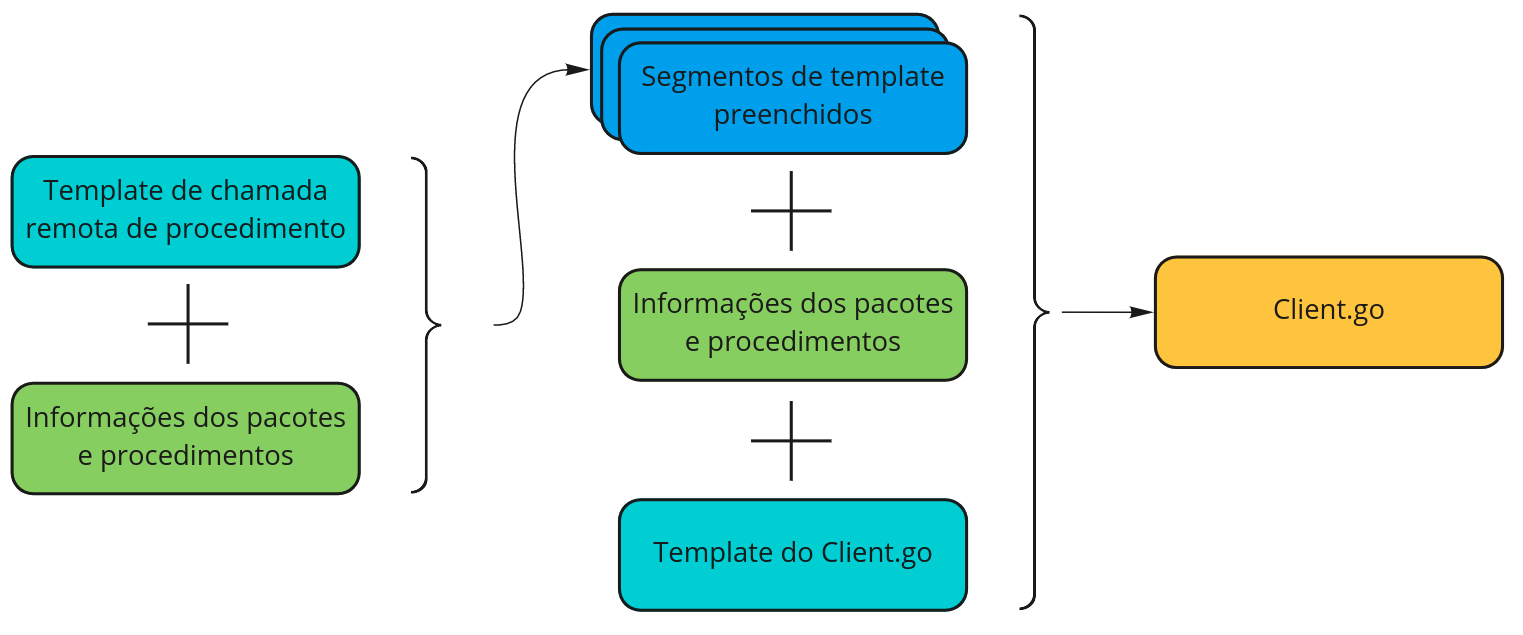
\includegraphics[width=\textwidth]{figuras/diagramas/cap3/arpc_compilador_client_go_gen.png}
    \label{fig:arpc_compiler_client_go_gen}
\end{figure}

Estes dados são incorporados em um \textit{template} de chamada remota de procedimento, de modo a gerar segmentos de código referente à função que deve ser invocada pelo cliente. Para cada segmento são substituídas no \textit{template} as informações coletadas anteriormente como: nome do pacote, nome do serviço, nome do procedimento, nome dos argumentos, tipo dos argumentos e tipo de retorno. O fluxograma do processo pode ser visto na Figura \ref{fig:arpc_compiler_client_go_gen}. 


O código gerado para cada procedimento é responsável por invocar a serialização dos argumentos, e chamar a função do controlador encarregada pelo envio dos dados serializados e do recebimento da resposta. Por fim, o código recebe o dado desserializado da resposta e o retorna para função que lhe invocou.

Para gerar o arquivo \textbf{Client.go} são incorporados os dados coletados do arquivo de IDL \textbf{*.arpc.go} e os segmentos de código gerados para os procedimentos no \textit{template} do serviço.

\subsection{Geração de código aRPC para servidores}

A geração do código dos procedimentos do serviço para o arquivo \textbf{Server.go} segue de forma análoga ao \textbf{Client.go}. Entretanto, existem algumas características distintas. No servidor, deve-se implementar uma interface que define todos os procedimentos oferecidos pelo serviço em uma \textit{struct}, em seguida essa \textit{struct} deve ser registrada no controlador. Dessa forma, além dos códigos que fazem o elo entre a implementação e serialização, o gerador constrói a interface do serviço a ser implementada pelo usuário, e uma função para efetuar o registro das \textit{structs} que estendem essa interface no controlador do servidor.

Apesar da interface de registro e da função que faz o elo entre o controlador e as implementações serem diferentes do arquivo do cliente, as informações necessárias para o preenchimento de seus \textit{template} são as mesmas, sendo a única diferença o seus códigos base.

Para gerar o arquivo \textbf{Server.go} são incorporados os dados coletados do arquivo de IDL \textbf{*.arpc.go} e os segmentos de código gerados para os procedimentos no \textit{template} do serviço.

\section{Uso do aRPC}

Como dito anteriormente, a proposta do aRPC é ser um protocolo rápido para HPC que impacte o mínimo possível na ergonomia da escrita da linguagem. Por essa razão o único momento onde o programador deve se preocupar com definições do aRPC é na inicialização da aplicação, onde ele fará a lógica de carregar os certificados, configuração do endereço de conexão, e configurações de \textbf{Channel}. Após definidos esses pontos, o cliente deve pegar uma referência para o serviço que se deseja executar e por fim chamar \textbf{controller.StartClient()}. A partir desse momento, todas as chamadas das funções de RPC e programação da aplicação seguem o fluxo usual de desenvolvimento. Para o servidor, ao invés de gerar uma referência para o serviço, o programador deve implementar a interface para o serviço e por fim, registrá-lo no controlador usando a função de registro do serviço gerada e então, deve executar \textbf{controller.StartServer()}. No Código \ref{alg:arpc_simple_service.go} é possível ver um exemplo dessa inicialização para um serviço simples. 

\includecode[Go]{Inicialização para o cliente em um serviço simples no aRPC} {alg:arpc_simple_service.go}{codigos/compilador/simple_service.go}{}


Vale ressaltar que todas as funções e procedimentos que utilizam rede, disponíveis no sistema do aRPC, fornecem um argumento opcional do tipo \textbf{ctx.Context} para gerenciamento do tempo limite e cancelamento de rotinas em execução. Assim, o programador pode escolher usar esses argumentos para ter mais controle da aplicação, ou omiti-los para um uso mais transparente do RPC.
